\documentclass[11pt,letterpaper]{spie}

% Commonly used packages
\usepackage{natbib}
\usepackage{epsfig}
\usepackage{graphicx}
\usepackage{pgf}  
\usepackage{caption}
\usepackage{multirow}
\usepackage[normalem]{ulem}
\usepackage{color}
\usepackage{pdfpages}
\usepackage[breaklinks,colorlinks=true, pdfstartview=FitV, linkcolor=blue, 
            citecolor=blue, urlcolor=blue]{hyperref}
\usepackage{rotating}
\usepackage{url}
\usepackage{amsmath}
\usepackage{amssymb}
\usepackage{bm}

% Bibliography
%\bibliographystyle{apj_w_etal}
%\citestyle{aa}
%/Users/jaguirre/Documents/Latex/journals.tex
%\pagenumbering{arabic}
%\pagestyle{plain}

\thispagestyle{empty}
% ------------------- Title and Author -----------------------------
\title{The Mini Radio Telescope (MRT):\\
Technical Update}
%\author{James Aguirre}

\begin{document}

\maketitle

The Mini Radio Telescope has now reached reasonable technical maturity, and we are working to make it completely robust for demonstrations, and capable of production in modest numbers.

The software is available publicly at \url{https://github.com/UPennEoR/MiniRadioTelescope}.

\begin{figure}[h]
\centering
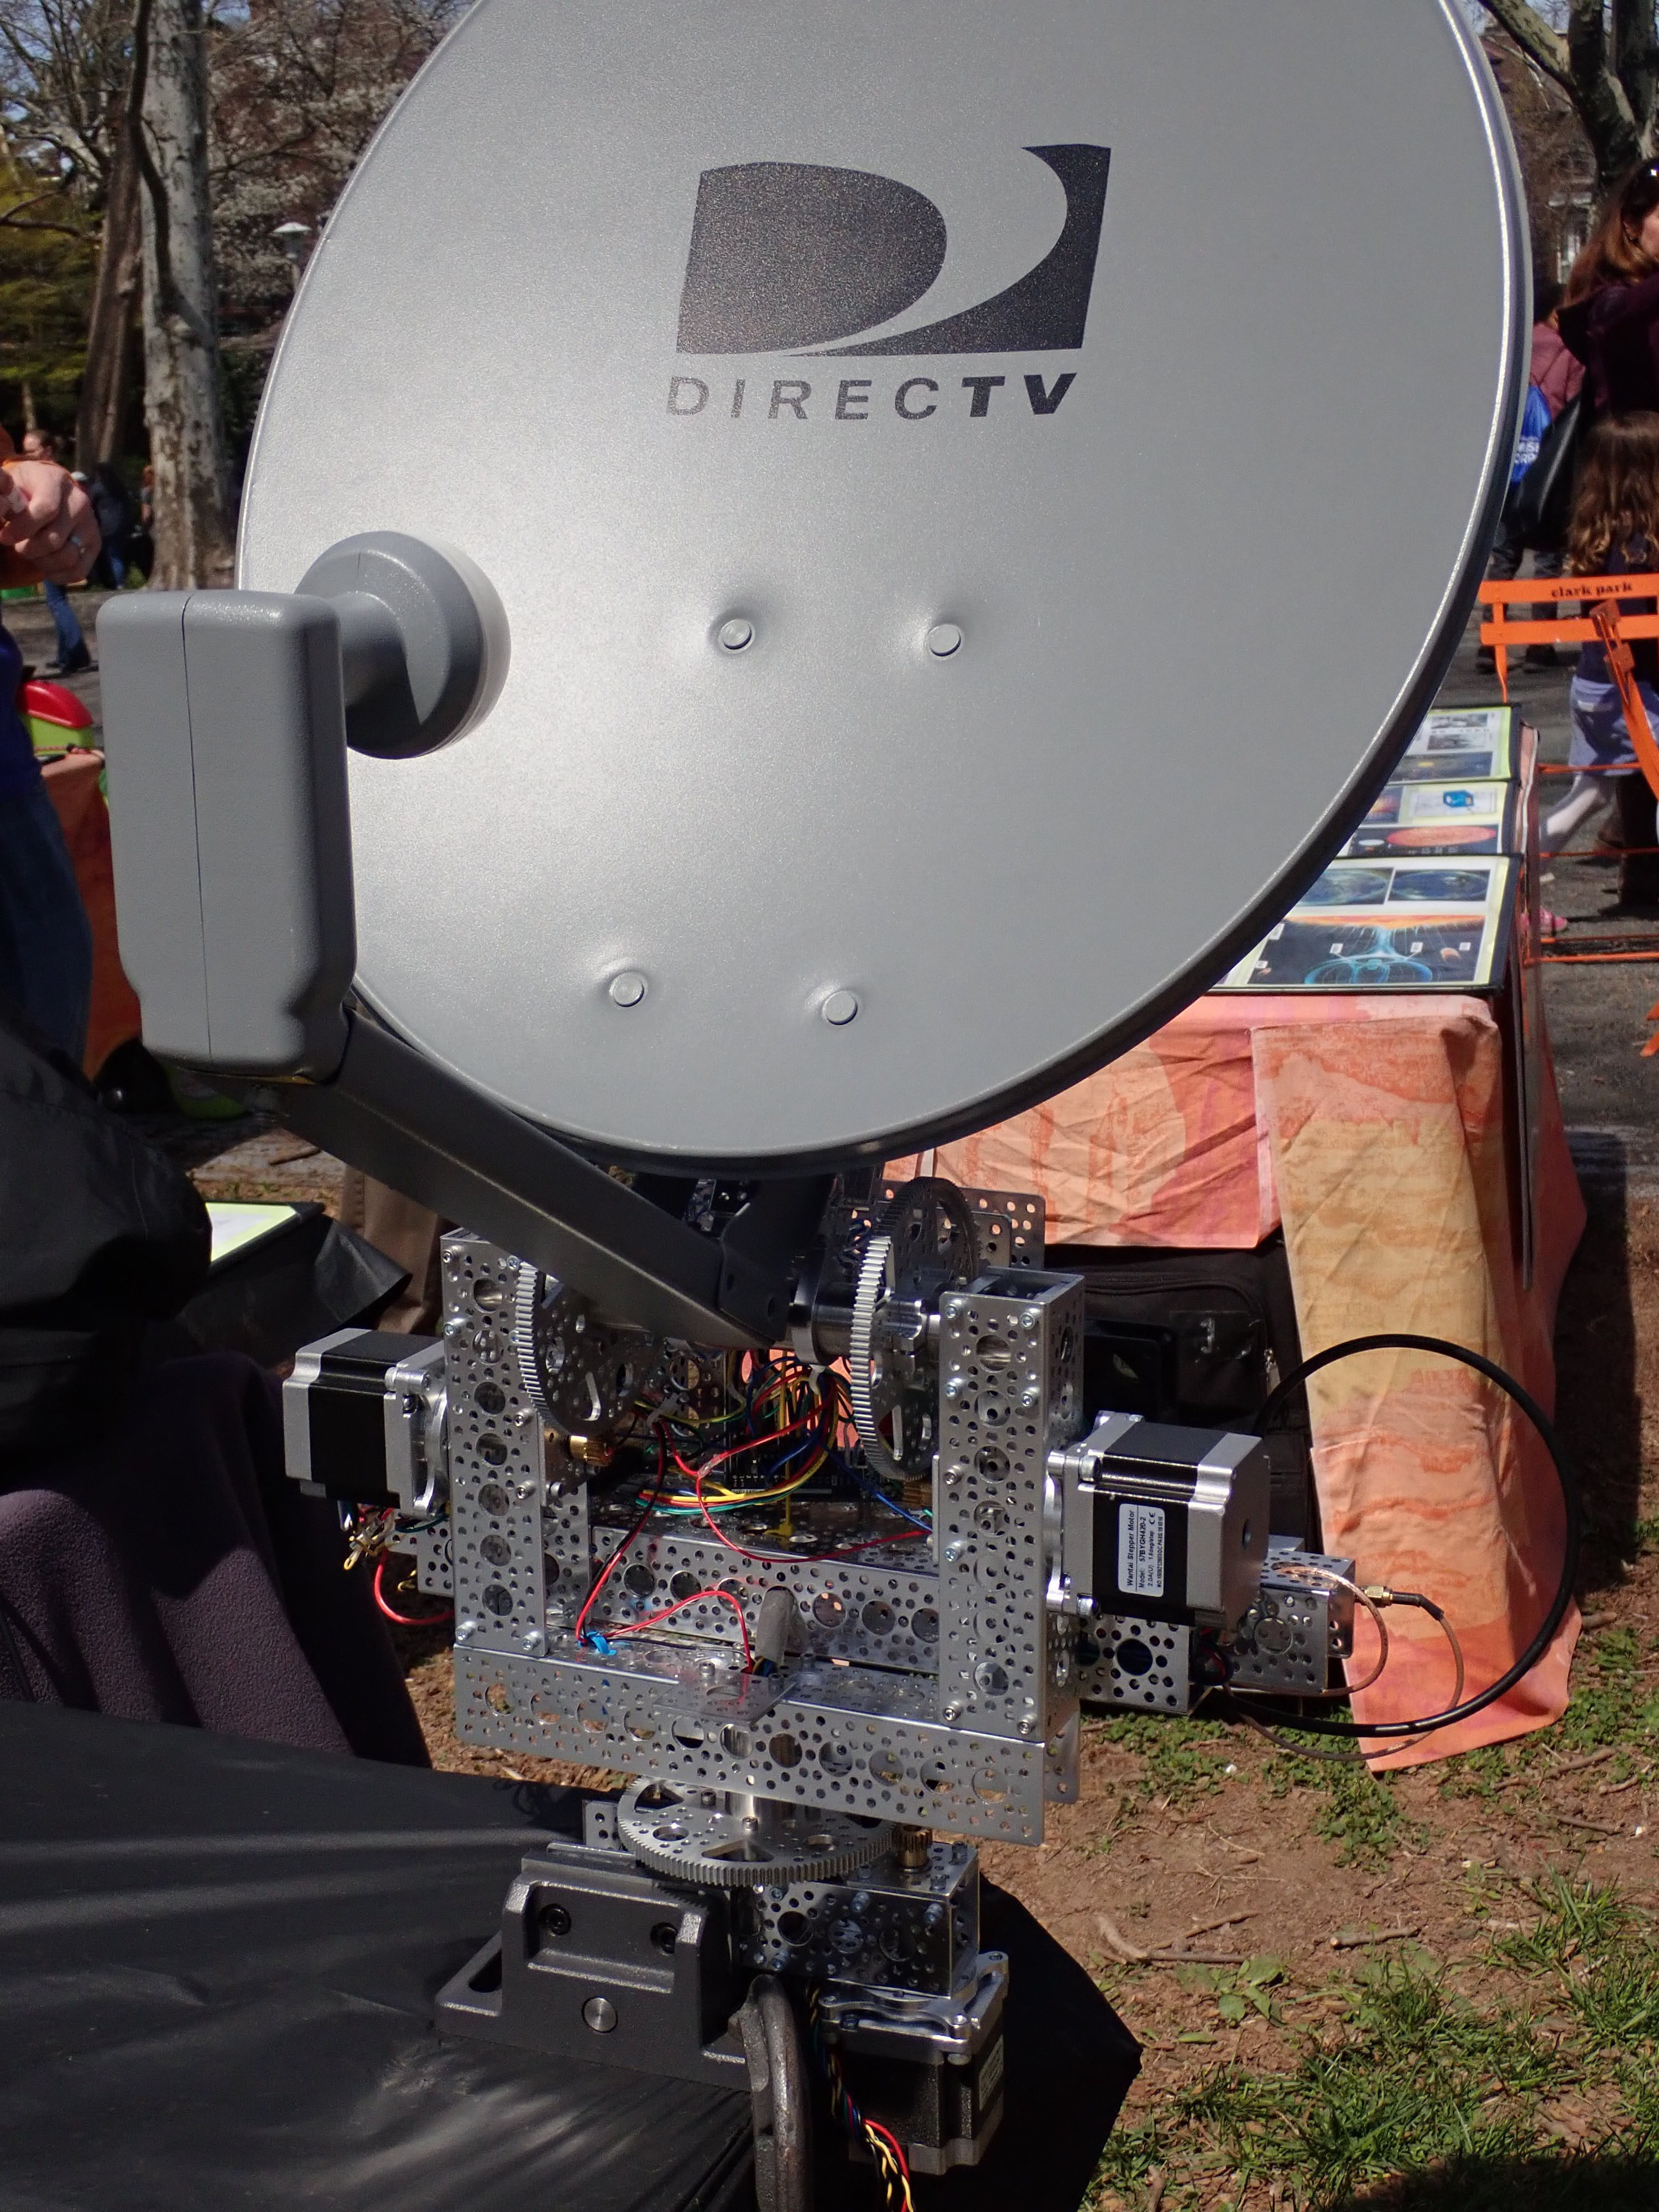
\includegraphics[height=6in]{MRT.jpg}
\vspace{5pt}
\caption{The Mini Radio Telescope in the spring of 2018.  All the components are commercially available and can be assembled with a minimal set of tools.}
\label{fig:Devices}
\end{figure}

\begin{figure}[h]
\centering
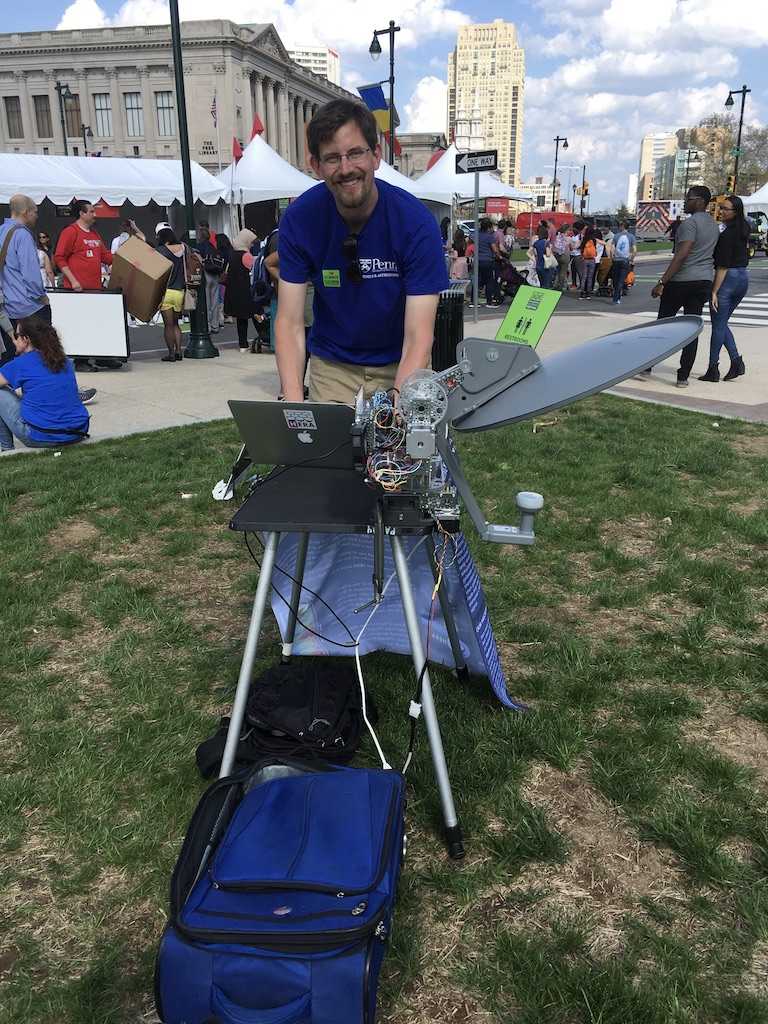
\includegraphics[width=6.5in]{PSFPortable.jpg}
\vspace{5pt}
\caption{The portable setup for the MRT on the Philadelphia Parkway for the Science Carnival.}
\label{fig:Devices}
\end{figure}

\begin{figure}[h]
\centering
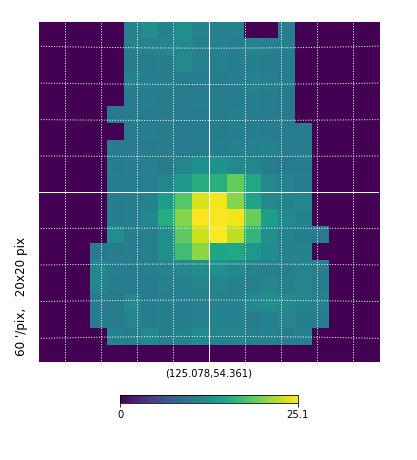
\includegraphics[width=3in]{mrt_sun_gnom.png}
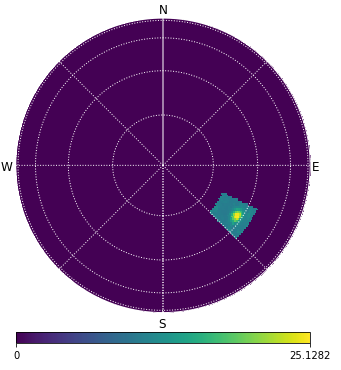
\includegraphics[width=3in]{mrt_sun_orth.png}
\vspace{5pt}
\caption{An MRT map of the sun.  Left: zoom in at the sun's location in altitude / elevation coordinates.   The resolution of the telescope ($5^\circ$) is larger than the true angular size of the sun ($0.5^\circ$).  Right: a view of the entire visible hemisphere showing the location of the mapped region.}
\label{fig:Sun}
\end{figure}

\begin{figure}[h]
\centering
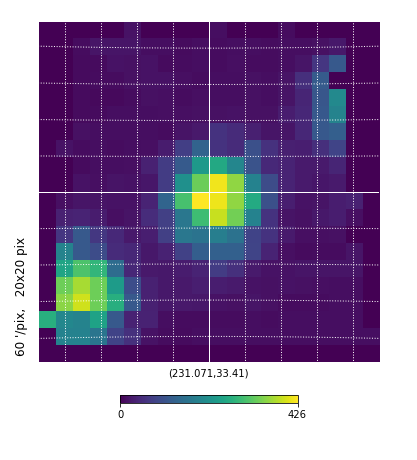
\includegraphics[width=3in]{mrt_sat_gnom.png}
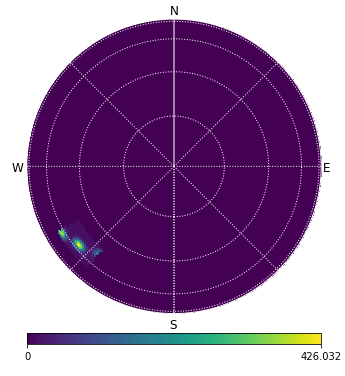
\includegraphics[width=3in]{mrt_sat_orth.png}
\vspace{5pt}
\caption{An MRT map of several geostationary satellites.  Same format as the Figure \ref{fig:Sun}.}
\label{fig:Satellites}
\end{figure}

%\bibliography{/Users/jaguirre/Documents/Latex/MasterReferences}

\end{document}


